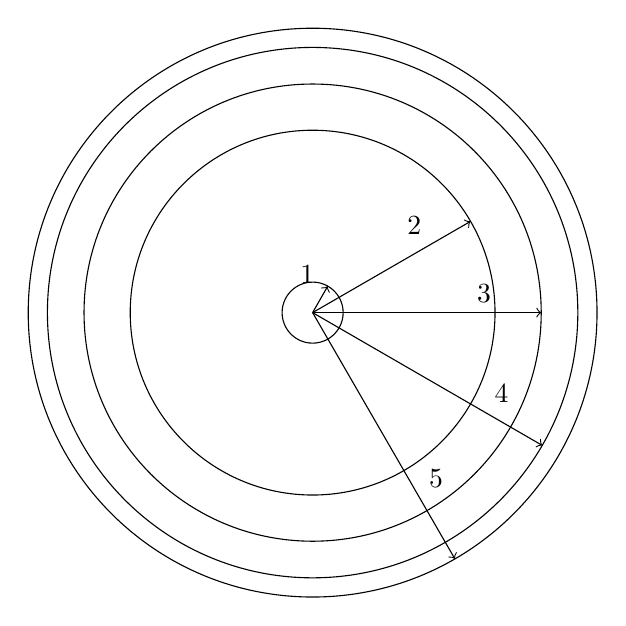
\begin{tikzpicture}[scale=6,auto]
        \draw (0,0) circle (0.06459);
      \draw[->] (0,0) -- node[pos=0.75] {1} (0.032,0.056);
      \draw (0,0) circle (0.38608);
      \draw[->] (0,0) -- node[pos=0.75] {2} (0.334,0.193);
      \draw (0,0) circle (0.48387);
      \draw[->] (0,0) -- node[pos=0.75] {3} (0.484,0.0);
      \draw (0,0) circle (0.56134);
      \draw[->] (0,0) -- node[pos=0.75] {4} (0.486,-0.281);
      \draw (0,0) circle (0.60198);
      \draw[->] (0,0) -- node[pos=0.75] {5} (0.301,-0.521);

      \end{tikzpicture}
      \begin{tikzpicture}
       \matrix [matrix of nodes]
      {
          Arrow & Radius (cm) & Material & \numrefheader \\
        1 & 0.06459 & \node[hyperlink node=mat_inconel]{Inconel}; & \ref{num:cr_plenum_spring}\\ 
        2 & 0.38608 & \node[hyperlink node=mat_helium]{Helium}; & \ref{num:CRthimIR}\\ 
        3 & 0.48387 & \node[hyperlink node=mat_SS304]{SS304}; & \ref{num:CRthimOR}\\ 
        4 & 0.56134 & \node[hyperlink node=mat_water]{Water}; & \ref{num:GTIRrad}\\ 
        5 & 0.60198 & \node[hyperlink node=mat_zirc]{Zircaloy}; & \ref{num:GTORrad}\\ 
      };
\end{tikzpicture}